\ifx\PREAMBLE\undefined
\documentclass{article}
\usepackage[format = hang, font = bf]{caption}
\usepackage{graphicx}
\usepackage{array}
\usepackage{amsmath}
\usepackage{mathtools}
\usepackage{boxedminipage}
\usepackage{listings}
\usepackage{makecell}%diagonal line in table
\usepackage{float}%allowing forceful figure[H]
\usepackage{xcolor}
\usepackage{amsfonts}%allowing \mathbb{R}
\usepackage{alltt}
\usepackage{url}
\def\UrlBreaks{\do\A\do\B\do\C\do\D\do\E\do\F\do\G\do\H\do\I\do\J\do\K\do\L\do\M\do\N\do\O\do\P\do\Q\do\R\do\S\do\T\do\U\do\V\do\W\do\X\do\Y\do\Z\do\[\do\\\do\]\do\^\do\_\do\`\do\a\do\b\do\c\do\d\do\e\do\f\do\g\do\h\do\i\do\j\do\k\do\l\do\m\do\n\do\o\do\p\do\q\do\r\do\s\do\t\do\u\do\v\do\w\do\x\do\y\do\z\do\0\do\1\do\2\do\3\do\4\do\5\do\6\do\7\do\8\do\9\do\.\do\@\do\\\do\/\do\!\do\_\do\|\do\;\do\>\do\]\do\)\do\,\do\?\do\'\do+\do\=\do\#\do\-}
\usepackage[breaklinks = true]{hyperref}
\lstset{language = matlab, breaklines = true, tabsize = 2, numbers = left, extendedchars = false, basicstyle = {\ttfamily \footnotesize}, keywordstyle=\color{blue!70}, commentstyle=\color{red!70}, frame=shadowbox, rulesepcolor=\color{red!20!green!20!blue!20}, numberstyle={\color[RGB]{0,192,192}}}

\begin{document}
\fi
\section{Machine learning diagnostics}
When the prediction of a hypothesis trained by a learning algorithm turns out to have unacceptable errors, a series of options are available as promising further actions to take:
\begin{enumerate}
\item Get more training examples.
\item Try smaller sets of features.
\item Try additional features.
\item Try polynomial features.
\item Adjusting value of regularization parameter $\lambda$.
\end{enumerate}
Rather than randomly try different approaches to improve the performance of the algorithm, it is worthwhile to implement machine learning diagnostics, which apply certain tests to figure out what is / isn't working and can thus provide guidance on what should be done next.
\subsection{Evaluate a hypothesis: test set}
Training the algorithm with all the examples available might end up overfitting the training set. To avoid such possibility, we can divide all examples into the {\bf training set} and the {\bf test set}. A typical choice is to put 70
\% of the examples in the training set and 30\% of the examples in the test set. Then a series of parameters $\theta$ can be learned from the training set by minimizing $J(\theta)$, after which the functionality of the algorithm can be measured by the test set error $J_{test}(\theta)$. For linear regression, we have 
$$J_{test}(\theta) = \frac{1}{2m_{test}}\sum\limits_{i=1}^{m_{test}}(h_{\theta}(x^{(i)}_{test}) - y^{(i)}_{test})^2$$
Similarly, for logistic regression, we have 
\begin{equation}\label{jtestlor}
J_{test}(\theta) = -\frac{1}{m_{test}}\sum\limits_{i=1}^{m_{test}}(y^{(i)}_{test}\log(h_{\theta}(x^{(i)}_{test})) +(1 - y^{(i)}_{test})\log(1-h_{\theta}(x^{(i)}_{test})))
\end{equation}
For logistic regression (i.e. 2-classification) problem, another way to define the test set error is 
$$J_{test}(\theta) = \frac{1}{m_{test}}\sum\limits_{i=1}^{m_{test}}err(h_{\theta}(x^{(i)}_{test}),y^{(i)}_{test})$$
in which 
\begin{equation*}
err(h_{\theta}(x,y) = \left\{
\begin{aligned}
1,&\text{ if }y = 0, h_{\theta}(x) \ge 0.5 \text{ or } y = 1, h_{\theta}(x) < 0.5\\
0,&\text{ otherwise}
\end{aligned}
\right.
\end{equation*}
\subsection{Model selection: cross-validation set}
In order to choose among different models (e.g. different degrees of polynomial), we need further partition of the examples. All examples should now be divided into 3 groups: {\bf training set}, {\bf cross-validation set} and {\bf test set}. Typically the percentages of the 3 groups are 60\%, 20\% and 20\%. 

For each training model candidate $h_{\theta}^{(i)}(x)$, we train a series of parameters $\theta^{(i)}$ by minimizing $J(\theta)$. Then we calculate the cross-validation set error $J_{cv}(\theta^{(i)})$ for them, in which 
$$J_{cv}(\theta) = \frac{1}{2m_{cv}}\sum\limits_{i=1}^{m_{cv}}(h_{\theta}(x^{(i)}_{cv}) - y^{(i)}_{cv})^2$$
for linear regression, and similar as \eqref{jtestlor} for logistic regression. Finally, the model that minimizes $J_{cv}(\theta)$ stands out, and its performance can be measured with the test set error.
\subsection{Bias \& variance}
When the training set is underfitted, the algorithm is said to have high bias, while when the training set is overfitted, it is said to have high variance. We will introduce methods to diagnose such problems.

In a specific linear regression problem, when higher order items are introduced into the hypothesis, the training set error (regularization not considered) will be reduced. However, too many high order items may cause overfit problem, which will increase the cross-validation set error. Figure \ref{biasvariance} depicts such trend.
\begin{figure}[H]
\centering
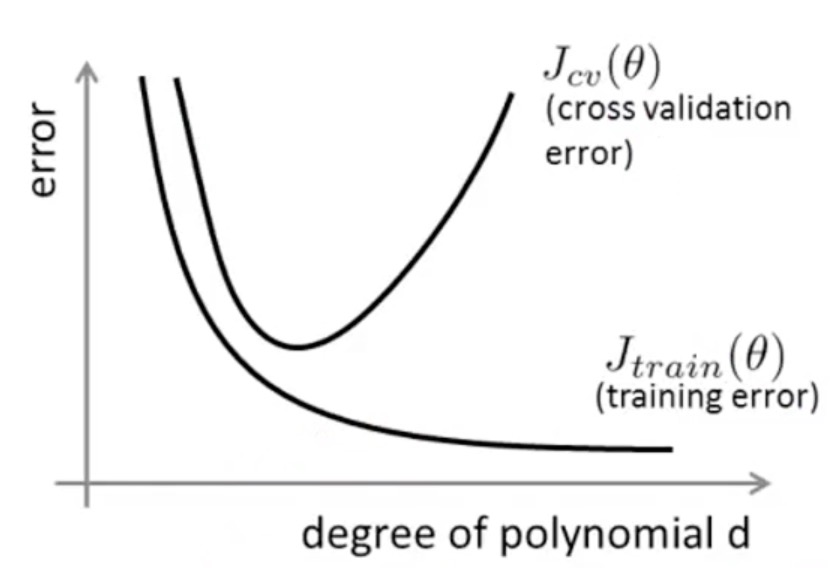
\includegraphics[width = 0.8\textwidth]{biasvariance.jpg}
\caption{Diagnosing bias and variance with errors: different polynomial degrees}\label{biasvariance}
\end{figure}
It is obvious that in a high bias (underfit) case, both $J_{cv}(\theta)$ and $J_{train}(\theta)$ are high, while in a high variance (overfit) case, $J_{cv}(\theta)$ is high but $J_{train}(\theta)$ is low.

We introduced regularization as the method to combat overfit, but the choice of the regularization parameter $\lambda$ can be subtle. It turns out that an appropriate $\lambda$ can be chosen following a criteria similar to that of model selection. Also, we can diagose bias and variance following the same rule stated above, as shown in Figure \ref{lambdachoice}. Here the $J_{train}(\theta)$ does not include the regularization item.
\begin{figure}[H]
\centering
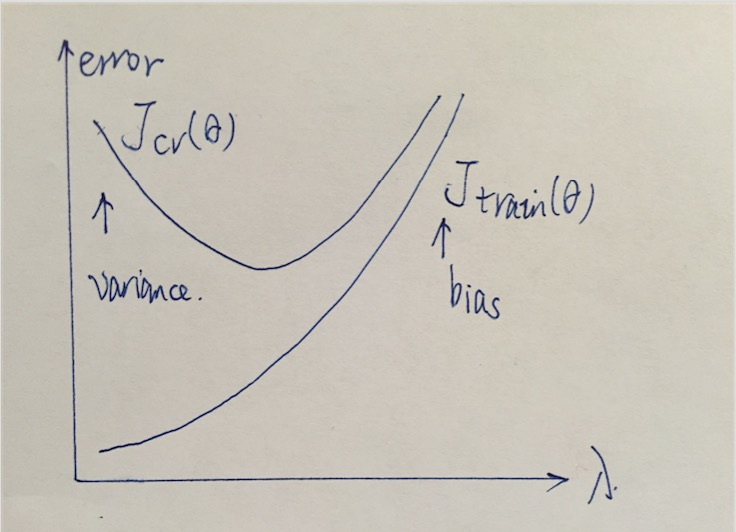
\includegraphics[width = 0.8\textwidth]{lambdachoice.jpg}
\caption{Diagnosing bias and variance with errors: different regularization parameter}\label{lambdachoice}
\end{figure}
\subsection{Learning curve}
Learning curve is the curve that depicts the variance of the training error and the cross-validation error with the training set size $m$. It can help estimate whether or not the performance of the algorithm will be improved by adding more examples into the training set.

When more examples are added into the training set, the hypothesis can no longer fit all examples well, thus the training error $J_{train}(\theta)$ will increase, whereas the hypothesis extends better towards new examples, thus the cross-validation error $J_{cv}(\theta)$ decreases. A typical learning curve is shown in Figure \ref{learningcurve}. 
\begin{figure}[H]
\centering
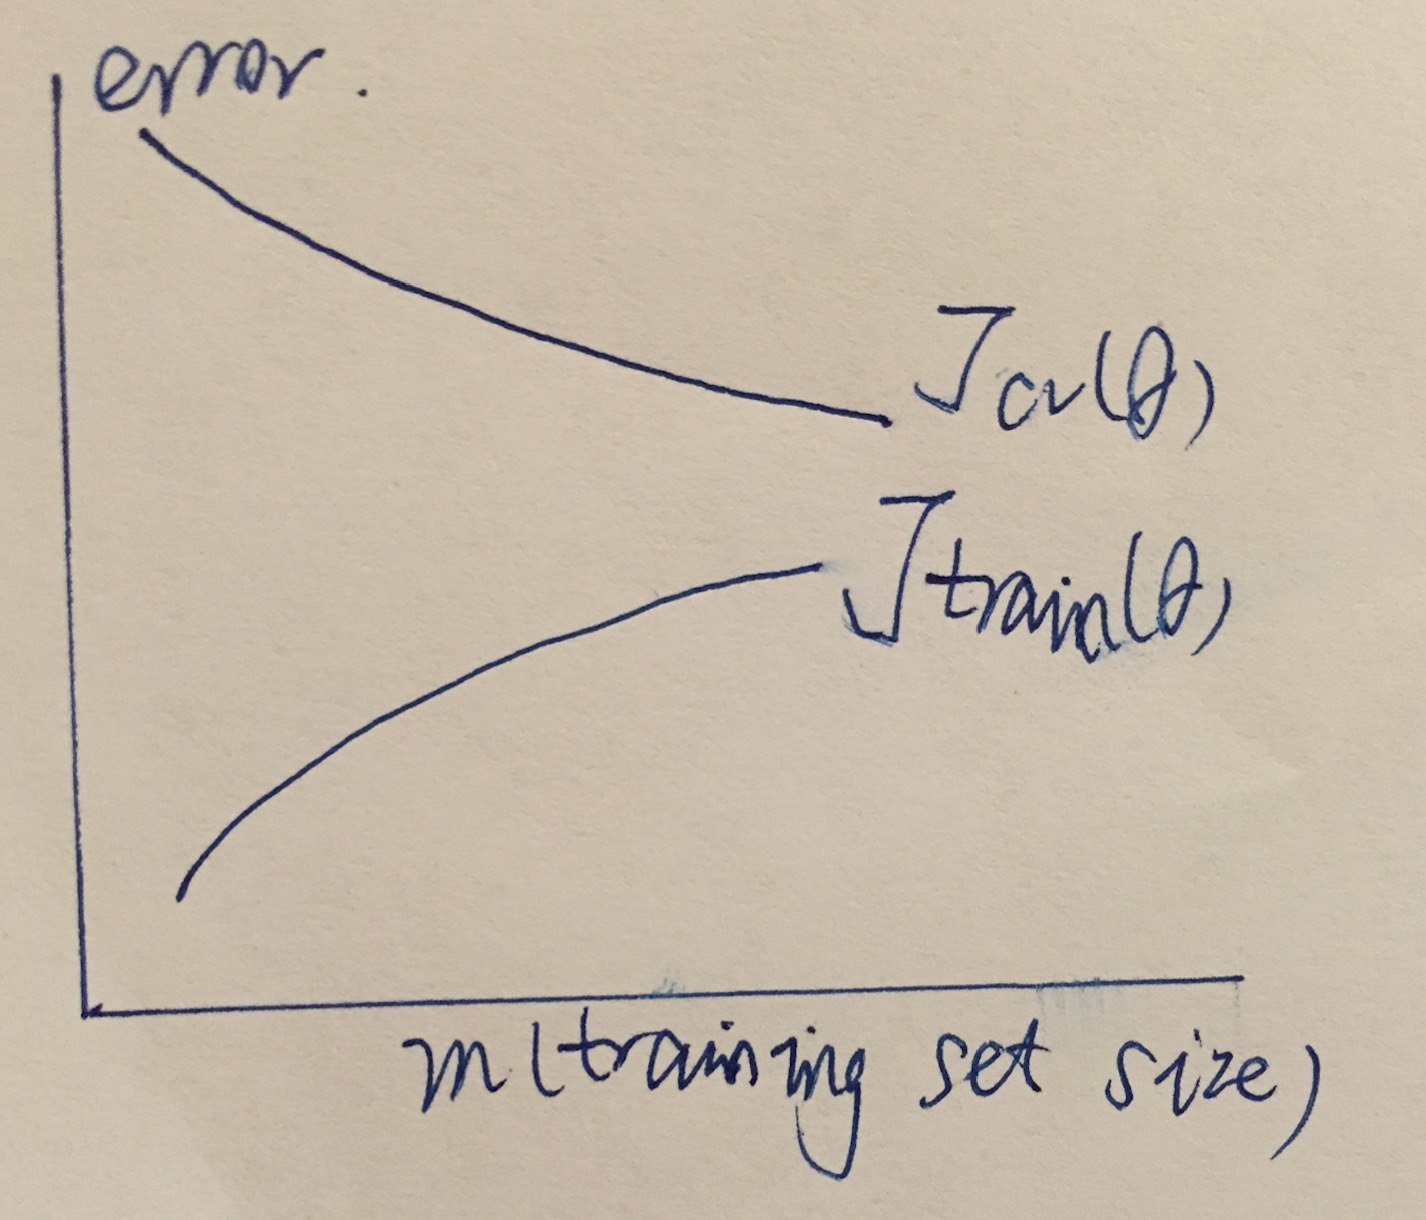
\includegraphics[width = 0.6\textwidth]{learningcurve.jpg}
\caption{A typical learning curve}\label{learningcurve}
\end{figure}

In a high-bias case, the examples are underfitted (e.g. trying to fit examples that follow a 5-degree polynomial with a straight line). Even if the size of the training set is increased, the hypothesis will still fail to correctly describe the relationship between the input and the output. Thus, both $J_{cv}(\theta)$ and $J_{train}(\theta)$ will be high, and they will be quite close to each other, as shown in Figure \ref{highbiascurve}. In this case, {\bf collecting more training examples is not likely to help.} Essential adjustment to the hypothesis should be made, i.e. adding more features.
\begin{figure}[H]
\centering
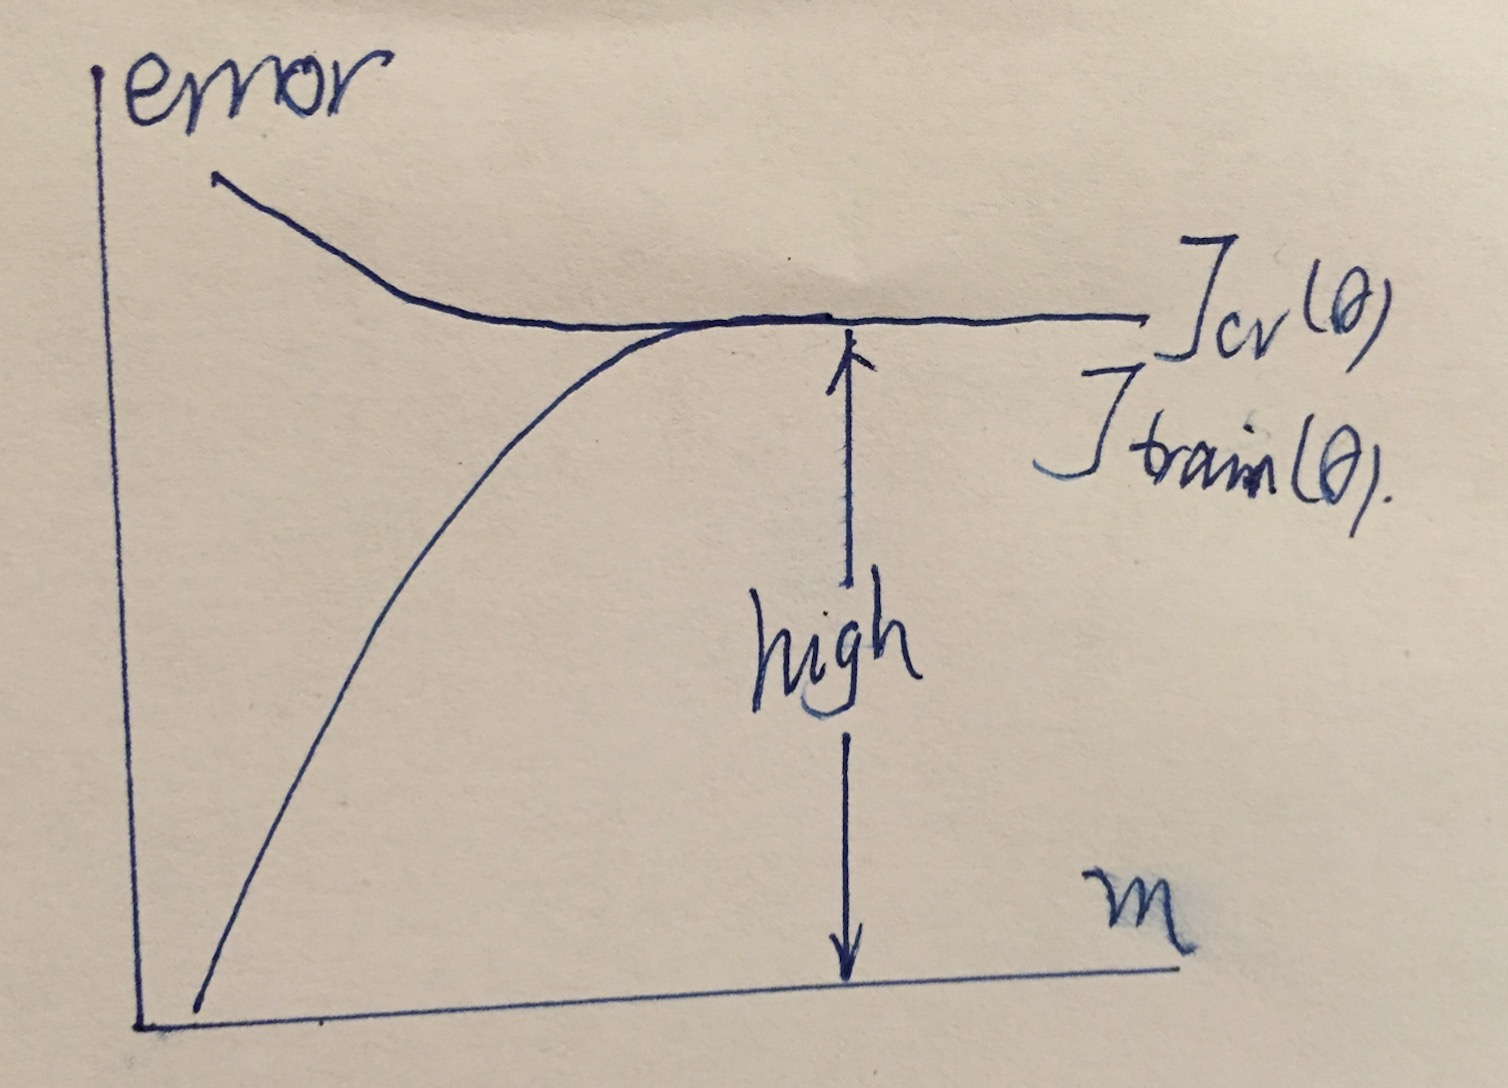
\includegraphics[width = 0.6\textwidth]{highbiascurve.jpg}
\caption{Learning curve with high bias}\label{highbiascurve}
\end{figure}

In a high variance case, the examples are overfitted. $J_{train}(\theta)$ is typically lower than $J_{cv}(\theta)$, as shown in Figure \ref{highvariancecurve}. If more examples are added to the training set, the training set becomes ``less overfitted'', thus $J_{train}(\theta)$ is likely to increase, while $J_{cv}(\theta)$ will decrease. In such case, 
{\bf collecting more training examples will help to improve the performance.}
\begin{figure}[H]
\centering
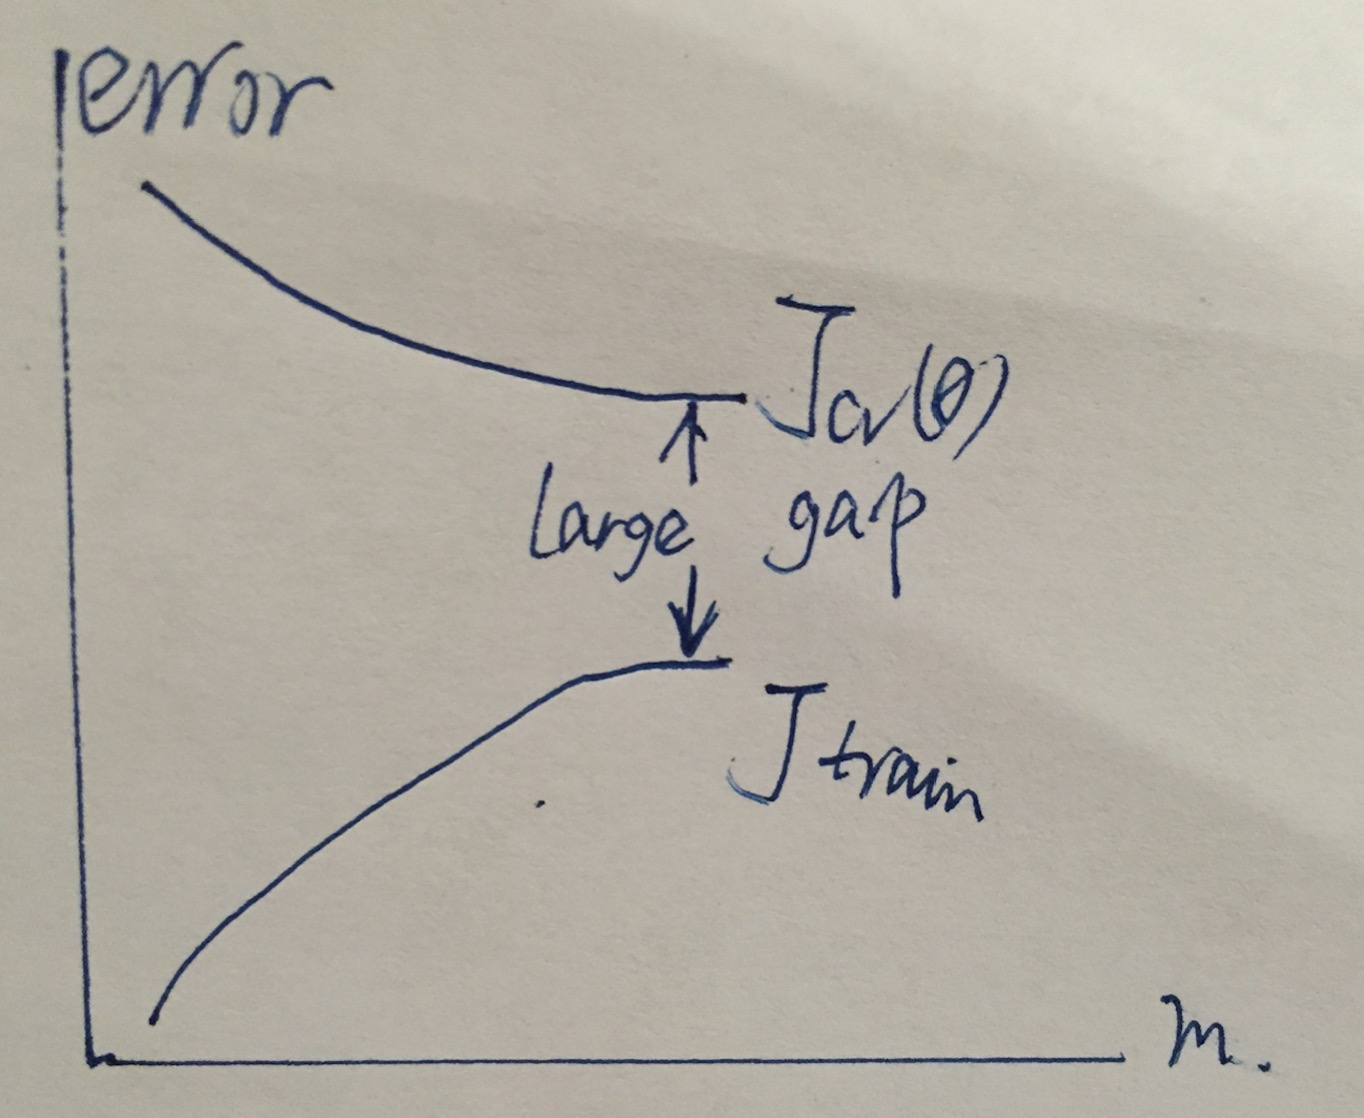
\includegraphics[width = 0.6\textwidth]{highvariancecurve.jpg}
\caption{Learning curve with high variance}\label{highvariancecurve}
\end{figure}
\subsection{Conclusion}
We will now conclude this section by providing the effects of the solutions to performance problems listed at the begining.
\begin{description}
\item [Get more training examples] fixes high variance
\item [Try smaller sets of features] fixes high variance
\item [Try additional features] fixes high bias
\item [Try polynomial features] fixes high bias
\item [Increase regularization parameter $\lambda$] fixes high variance
\item [Decrease regularization parameter $\lambda$] fixes high bias
\end{description}
\section{Machine learning system design}
When designing a machine learnig system, a bunch of different options are available for choice to achieve better performance. Take the example of an email spam classifier, we can: 
\begin{itemize}
\item Collect large amount of data.
\item Develop sophisticated features based on email routing information, e.g. email header.
\item Develop sophisticated features for message body, e.g. treating `discount' and `discounts', `dealer' and `Dealer' as the same word, ignoring punctuations, etc.
\item Develop sophisticated algorithm to detect misspellings, e.g. `magaz1ne', `m0rtgage', etc.
\end{itemize}
Rather than randomly making a choice based on gut feeling, systematic analysis methods are available to help choose the best option.
\subsection{Error analysis}
A recommended approach to a machine learning problem is as follows. Start with a ``quick and dirty'' version of the algorithm easy to implement. Implement it and test it on the cross-validation set. Plot learning curves to decide if more data or more features are needed. Then conduct what we call {\bf error analysis}: manually examine examples in c-v set on which the algorithm made errors, and try to figure out any systematic trend of such examples. Based on the trends, add new features to the model and see if it helps.
\subsection{Handling skewed data}
Take the cancer classification as an example. If we have a learning algorithm that diagnoses the test set with 1\% error, i.e. 99\% of the diagnostics it make are correct, it seems to be a good algorithm. However, provided that only 0.5\% of the patients in the training set have cancer, this algorithm is far from satisfactory. Actually, a dumb classifier that always outputs $y=0$ (no cancer) appears to have better performance. Obviously, in such case, classification error, or classification accuracy, is no longer an appropriate metric of the performance of the algorithm. 

\begin{table}[H]
\centering
\caption{Definitions for skewed data error metrics}\label{skeweddefs}
\begin{tabular}{c|c|c}
\diaghead(3,-1){\hskip2.2cm}%
{\\Predicted}{Actual}
&1&0\\\hline
1&True Positive&False Positive\\\hline
0&False Negative&True Negative\\
\end{tabular}
\end{table}
Table \ref{skeweddefs} provides some useful definitions for skewed data error metrics. If the actual class is 1 and the algorithm predicts 1, we say that the algorithm has made a true positive prediction, etc. Now we can define the {\bf precision} and the {\bf recall} of the algorithm.
\begin{equation}
\begin{split}
\text{Precision} = \frac{\text{True Positive}}{\text{True Positive} + \text{False Positive}}\\
\text{Recall} = \frac{\text{True Positive}}{\text{True Positive} + \text{False Negative}}\\
\end{split}
\end{equation}
Clearly, precision is the percentage of patients who actually have cancer among patients diagnosed to have cancer, while recall is the percentage of patients who are diagnosed to have cancer among patients who actually have cancer.

With precision and recall defined, we can introduce the tradeoff between them. Normally we predict $y=1$ when $h_{\theta}(x) \ge 0.5$ and $y=0$ when $h_{\theta}(x) < 0.5$. If we want to predict $y=1$ only when very confident, we can increase the threshold for prediction, e.g. to 0.9. Obviously this will increase the precision but decrease the recall. On the contrary, if we want to alert more patients possible to have cancer, we can decrease the threshold, say to 0.3, and we will end up with lower precision but higher recall.

Taking both precision and recall into account, we define the $F_1$ score of the algorithm
\begin{equation}
F_1 = \frac{2PR}{P+R}
\end{equation}
and use it as a measurement of the performance of the algorithm. Generally, an algorithm with a better $F_1$ score has better overall performance.
\subsection{Data}
Sufficient and appropriate data is essential to the performance of the algorithm. We should always ensure that the features we use include {\bf enough} information to predict the output correctly. A useful test to determine whether the information is enough is to ask ourselves: is a human expert in this field capable of making a confident predication of the output based on the information we provide?

If we are using low-bias algorithms, e.g. neural network with a lot of hidden layers or a linear regression with a lot of feature, large amount of data will help avoid overfitting and is thus usually preferable.
\ifx\PREAMBLE\undefined
\end{document}
\fi